%
\begin{figure*}[!t]
  \centering
  \subfigure{
    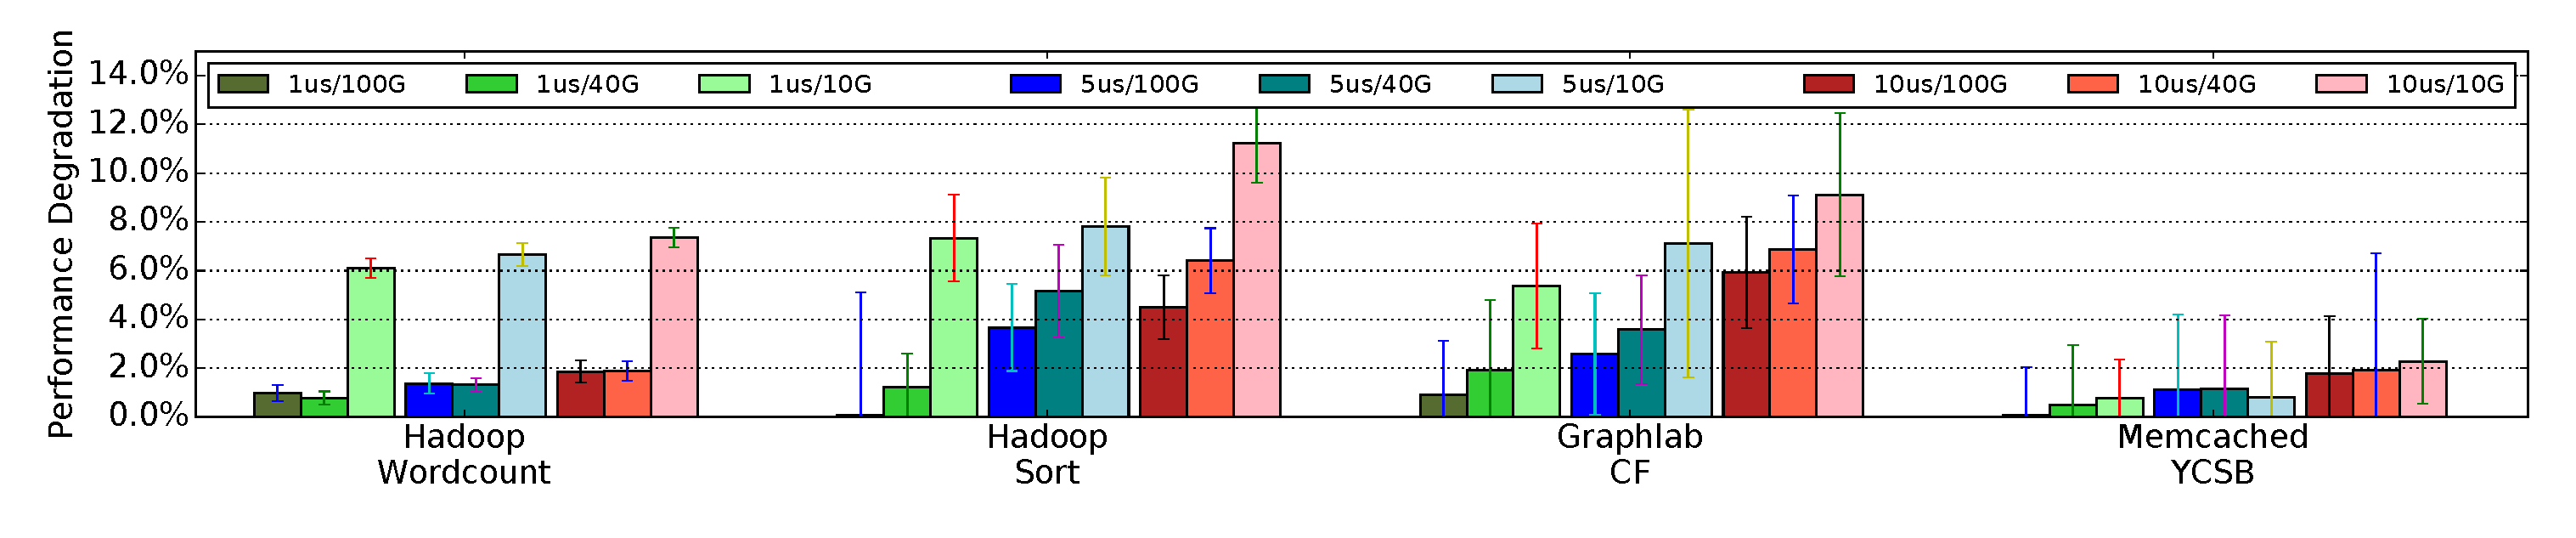
\includegraphics[width=\textwidth]{img/vary_latency_bw.eps}  
  }
  \subfigure{
    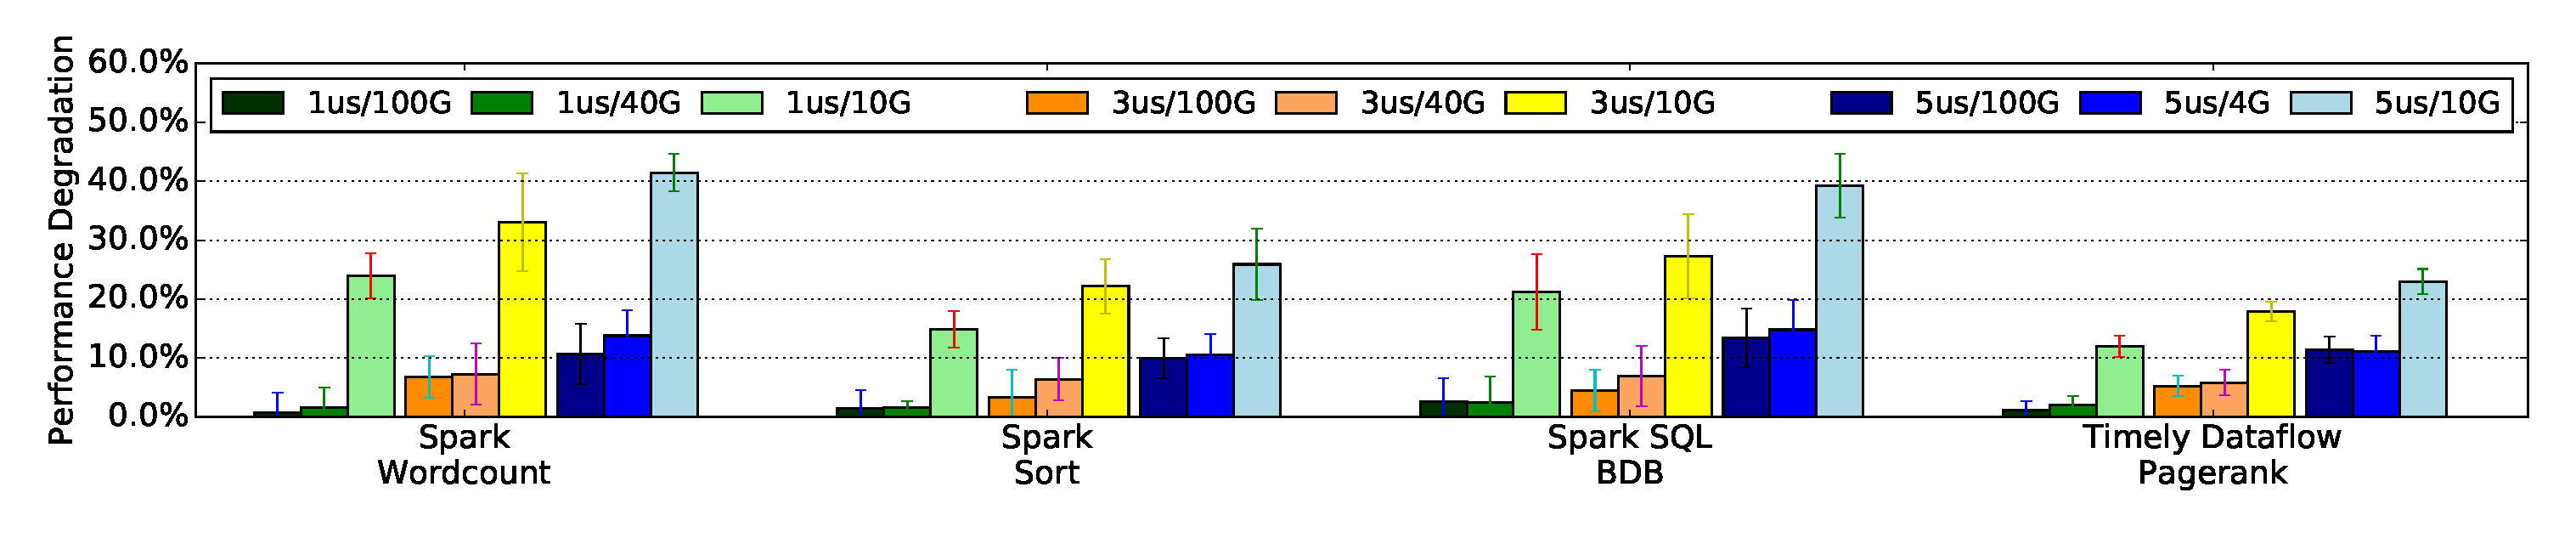
\includegraphics[width=\textwidth]{img/vary_latency_bw_high.eps}
  }
  \caption{\small{Comparison of application-level performance in disaggregated datacenters with respect to existing server-centric architectures for different latency/bandwidth configurations and $25\%$ local memory on CPU blades --- \dolphin apps (top) and \shark apps (bottom). To maintain application-level performance within reasonable performance bounds ($\sim 5\%$ on an average), \dolphin require $5\mu$s end-to-end latency and $40$Gbps bandwidth, and \shark apps require $3\mu$s end-to-end latency and $40-100$Gbps bandwidth. See \S\ref{ssec:rr} for detailed discussion.}}
  \label{fig:latb}
\end{figure*}
%
%\vspace{-0.1in}
\section{Network Requirements}
\label{sec:requirements}
%\vspace{-0.05in}
We start by evaluating network latency and bandwidth requirements for disaggregation.
We describe our evaluation methodology (\S \ref{ssec:rmethod}), present our results (\S \ref{ssec:rr}) and then discuss their implications (\S \ref{ssec:rtt}). 

%\vspace{-0.1in}
\subsection{Methodology}
\label{ssec:rmethod}
%\vspace{-0.05in}
%\rc{reviewer: why not a hardware simulator}
In \dis, traffic between resources that was contained within a server is now carried on the ``external'' network. As with other types of interconnects, the key requirement will be low latency and high throughput to enable this disaggregation. We review the forms of communication between resources within a server in Table~\ref{tab:tech} to examine the feasibility of such a network. As mentioned in \S\ref{sec:summary}, CPU-to-CPU cache coherence traffic does not cross the external network.
For I/O traffic to storage devices, the current latency and bandwidth requirements are such that we can expect to consolidate them into the network fabric with low performance impact, \revisionb{assuming we have a 40Gbps or 100Gbps network}. 
Thus, the dominant impact to application performance will come from CPU-memory disaggregation; hence, we focus on evaluating the network bandwidth and latency required to support remote memory. 

As mentioned earlier, we assume that remote memory is managed at the page granularity, in conjunction with virtual memory page replacement algorithms implemented by the hypervisor or operating system.
For each paging operation there are two main sources 
of performance penalty: i) the software overhead for trap and page eviction and ii) the time to transfer pages over the network. 
Given our focus on network requirements, we only consider the latter in this paper (modulo a brief discussion on current 
software overheads later in this section).

\paragraphb{Applications}
% We conduct a series of experiments to examine how network latency and bandwidth affect application performance with remote memory accesses (which we emulate as described below). 
We use workloads from diverse applications running on real-world and benchmark datasets, as shown in Table~\ref{tab:workloads}. 
\eat{
\sr{Old short-and-sweet text}
We take these applications as is rather than seek to optimize them for \dis; this represents a worst-case for the network, as \dis-driven application modifications could lessen the network requirements. 
}
%\sr{New long-and-gory text}
We elaborate briefly on our choice to take these applications as is, rather than seek to optimize them for \dis. Our focus in this paper is on understanding whether and why networking might gate the deployment of \dis.  
For this, we are interested in the degradation that applications might suffer if they were to run in \dis. We thus compare the performance of an application in a server-centric architecture to its performance in the disaggregated context we consider here (with its level of bandwidth and local memory). 
This would be strictly worse than if we compared to the application's performance if it had been rewritten for this disaggregated context. Thus, legacy (i.e., server-centric) applications represent the worst-case in terms of potential degradation and give us a lower bound on the network requirements needed for disaggregation (it might be that rewritten applications could make due with lower bandwidths). 
Clearly, if new networking technologies exceed this lower bound, then all applications (legacy and ``native'' \dis) will benefit. Similarly, new programming models designed to exploit disaggregation can only improve the performance of all applications. 
The question of how to achieve improved performance through new technologies and programming models is an interesting one but beyond the scope of our effort and hence one we leave to future work. 


%These workloads constitute a wide variety of application domains including off-disk batch processing (Hadoop), in-memory batch processing (Spark), graph processing (GraphLab) and point queries (memcached).




\paragraphb{Emulating remote memory} 
\revisionb{We run the following applications unmodified with $8$ threads and reduce the amount of local memory directly accessible by the applications. 
To emulate remote memory accesses, we implement a special swap device backed by the remaining physical memory rather than disk. 
This effectively partitions main memory into ``local'' and ``remote'' portions where existing page replacement algorithms control when and how pages are transferred between the two. 
We tune the amount of ``local'' memory by configuring the size of the swap device.
When a page fault occurs, the page is not actually swapped over the network, instead, it is swapped to the remaining part of the memory on the same machine.
However, we intercept all page faults and inject artificial delays to emulate network round-trip latency and bandwidth for each paging operation. 


We measure relative application-level performance on the basis of job completion time as compared to the zero-delay case. 
Thus, our results do not account for the delay introduced by software overheads for page operations and should be interpreted as \emph{relative} performance degradations over different network configurations. %, not the absolute performance of disaggregation.
Note too that the delay we inject is purely an artificial parameter and hence does not realistically model queuing delays that may result from network congestion caused by the extra traffic due to disaggregation; we consider network-wide traffic and effects such as congestion in \S\ref{sec:existing}.
}


%
\paragraphb{Testbed}
Each application operates on $\sim125$GB of data equally distributed across an Amazon EC2 cluster comprising $5$ m3.2xlarge servers. Each of these servers has $8$ vCPUs, $30$GB main memory, $2 \times 80$GB SSD drives and a $1$Gbps access link bandwidth.
We enabled EC2's Virtual Private Network (VPC~\cite{vpc}) capability in our cluster to ensure no interference with other Amazon EC2 instances. 

We verified that \texttt{m3.2xlarge} instances' $1$Gbps access links were not a bottleneck to our experiment in two ways. 
First, in all cases where the network approached full utilization, CPU was highly utilized, indicating that the CPU was not blocked on network calls.
Next, we ran our testbed on \texttt{c3.4xlarge} instances with $2$Gbps access links (increased network bandwidth with roughly the same CPU). We verified that even with more bandwidth, all applications for which link utilization was high maintained high CPU utilization.
\revisionb{This aligns with the conclusions drawn in ~\cite{kay-nsdi15}.}
 
\revision{We run batch applications (Spark, Hadoop, Graphlab, and Timely Dataflow) in a cluster with 5 worker nodes and 1 master node; the job request is issued from the master node.
For point-query applications (memcached, HERD), requests are sent from client to server across the network. 
All applications are multi-threaded, with the same number of threads as cores.
To compensate for the performance noise on EC2, we run each experiment 10 times and take the median result.
}
\begin{figure}[t]
  \centering
    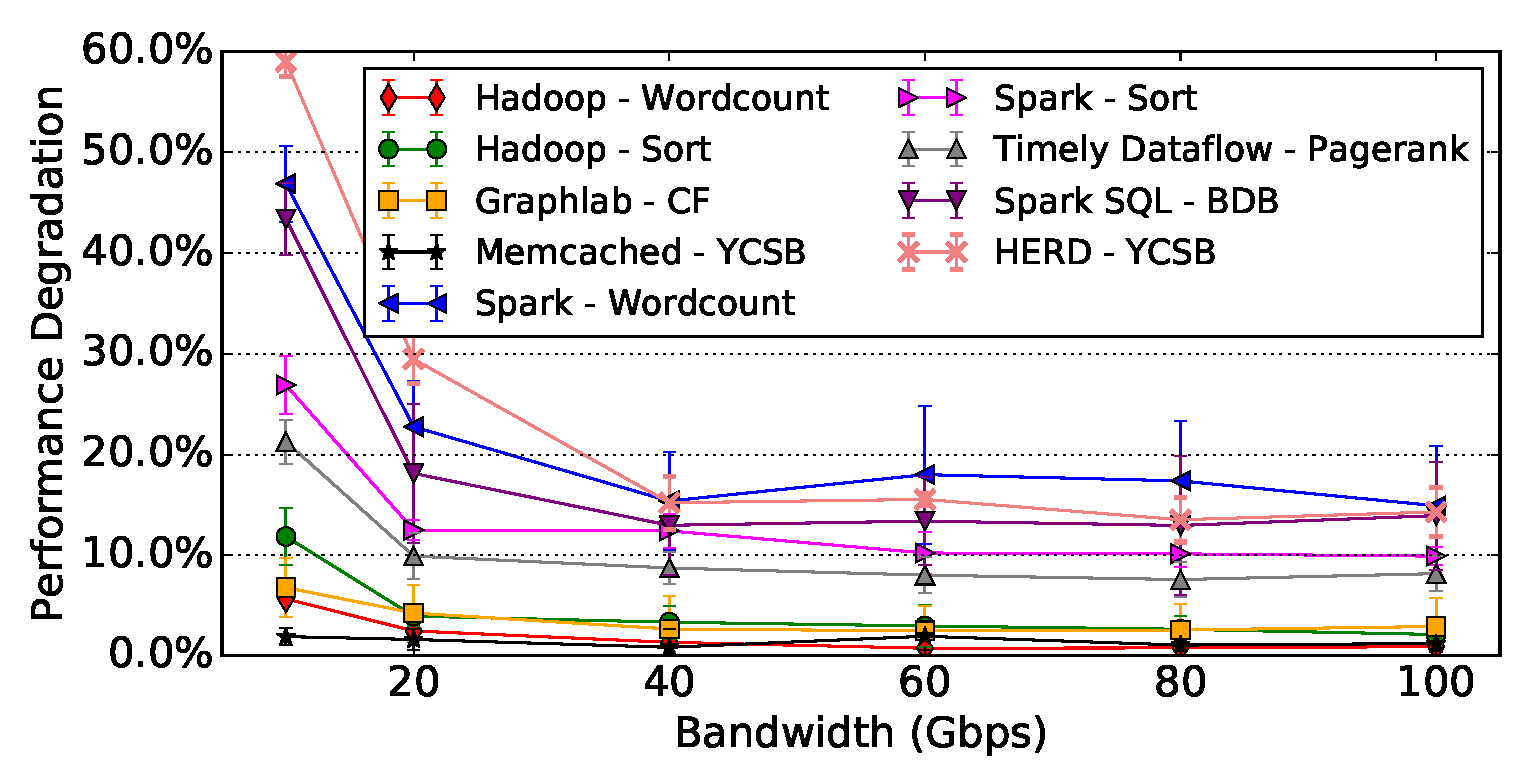
\includegraphics[width = \columnwidth]{img/fix_latency_vary_bw.eps} 
  \caption{\small{Impact of network bandwidth on the results of Figure~\ref{fig:latb} for end-to-end latency fixed to $5\mu$s and local memory fixed to $25\%$.}}% Beyond $40$Gbps, the network bandwidth has little or no impact on relative (disaggregated versus server-centric) application-level performance.}}
  \label{fig:impbw}
\end{figure}
%
%\vspace{10em}
%
\begin{figure}[t]
  \centering
    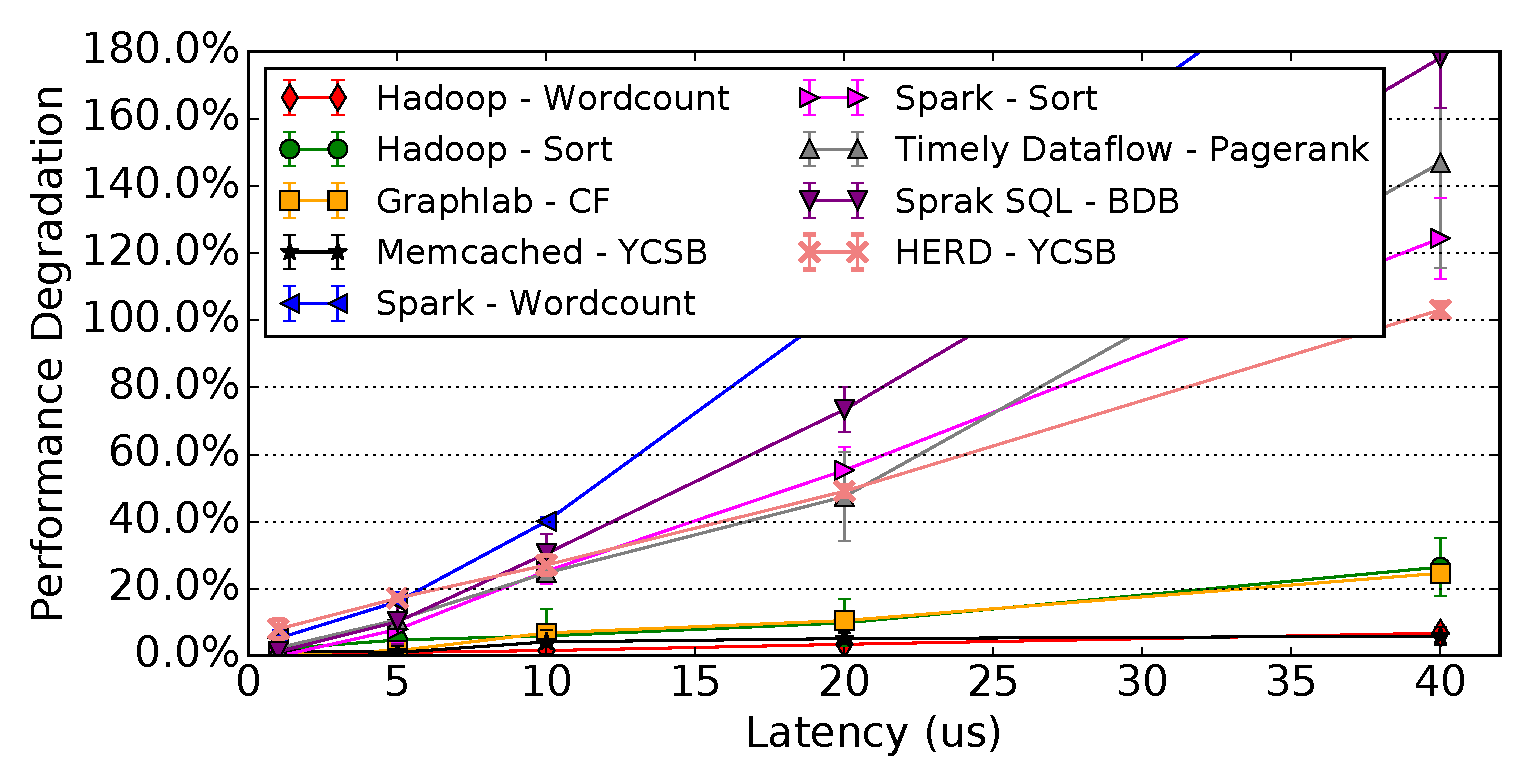
\includegraphics[width=\columnwidth]{img/fix_bw_vary_latency.eps} 
  \caption{\small{Impact of network latency on the results of Figure~\ref{fig:latb} for bandwidth fixed to $40$Gbps and local memory fixed to $25\%$. }} %Sharks are extremely sensitive to network latencies, while dolphins remains largely insensitive.}}
  \label{fig:impl}
\end{figure}
%
%\vspace{10em}
%
\begin{figure}[t]
  \centering
    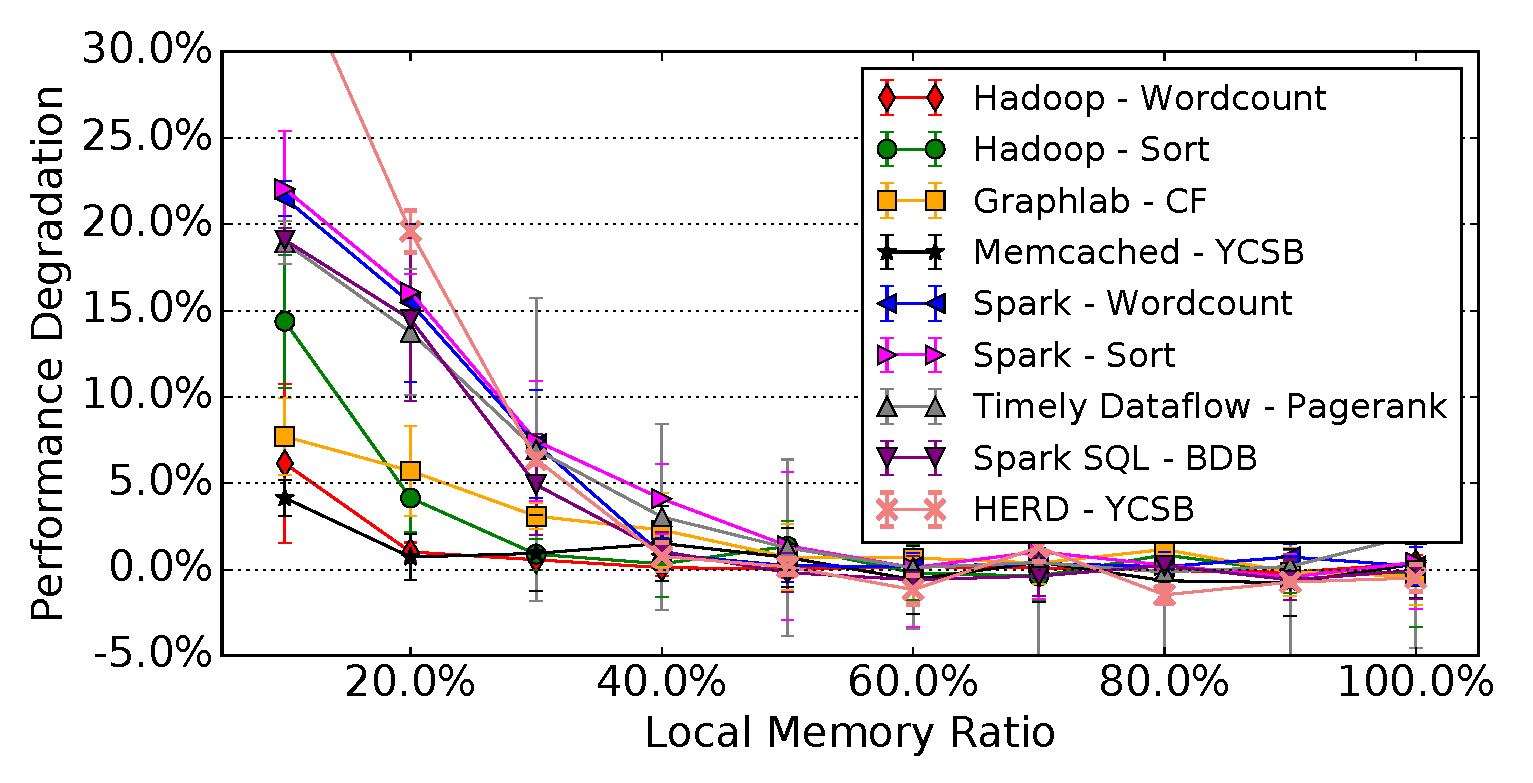
\includegraphics[width=\columnwidth]{img/vary_remote_mem.eps} 
  \caption{\small{Impact of ``local memory'' on the results of Figure~\ref{fig:latb} for end-to-end latency fixed to $5\mu$s and network bandwidth $40$Gbps. Negative values are due to small variations in timings between runs.}} %Local memory has significant impact on the performance of sharks and noticeable impact on dolphins (at least until $40\%$). Beyond $35\%$ local memory, both sharks and dolphins achieve performance within reasonable bounds. This could be reduced to $30\%$ for lower latency and/or higher bandwidth configurations (see Table~\ref{tab:rmem}).}}
  \label{fig:impb}
\end{figure}
%
%\vspace{20em}
%
\begin{table}[t]
    \centering
    \small
    \begin{tabular}{c|c|c}
    \textbf{Network Provision} & \textbf{\shark} & \textbf{\dolphin}\\
    \hline\hline
    $5\mu$s, $40$Gbps & $35$\% & $20$\%\\\hline
    $3\mu$s, $100$Gbps & $30$\% & $15$\%\\\hline\hline
    \end{tabular}
    \caption{\small{\shark apps require slightly higher local memory than \dolphin apps to achieve an average performance penalty under $5\%$ for various latency-bandwidth configurations.}}
    \label{tab:rmem}
\end{table}
%
%
\begin{figure*}[t]
    \centering
    \subfigure[Swap Bandwidth Utilization]{
        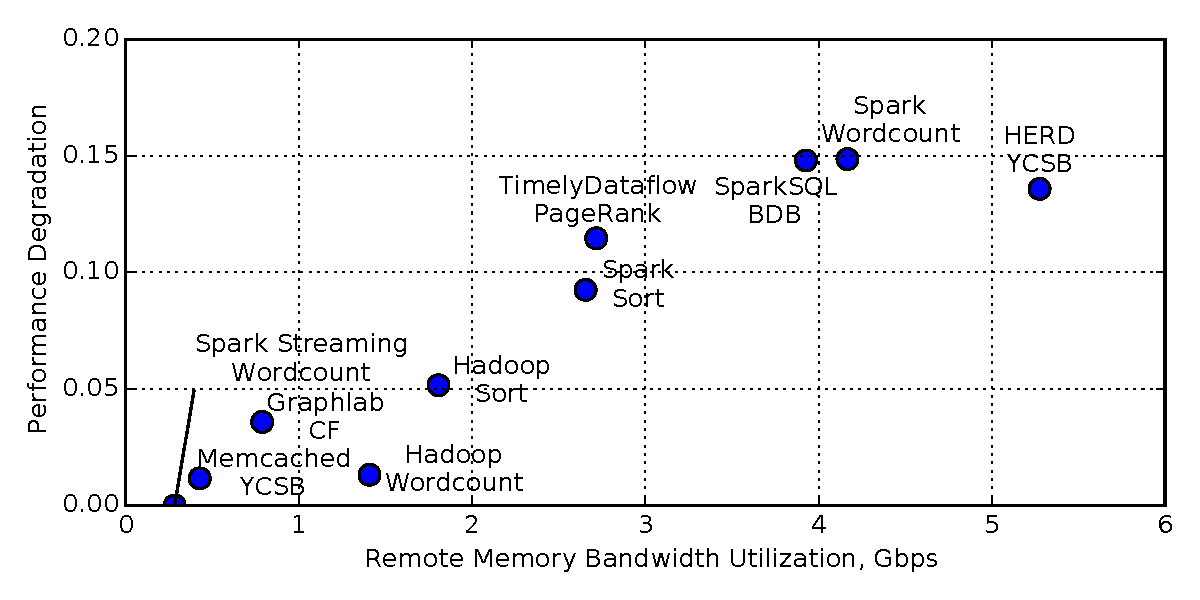
\includegraphics[width=0.95\columnwidth]{img/swap_bandwidth}
        \label{fig:swapband}
    }
    \subfigure[Memory Bandwidth Utilization]{
        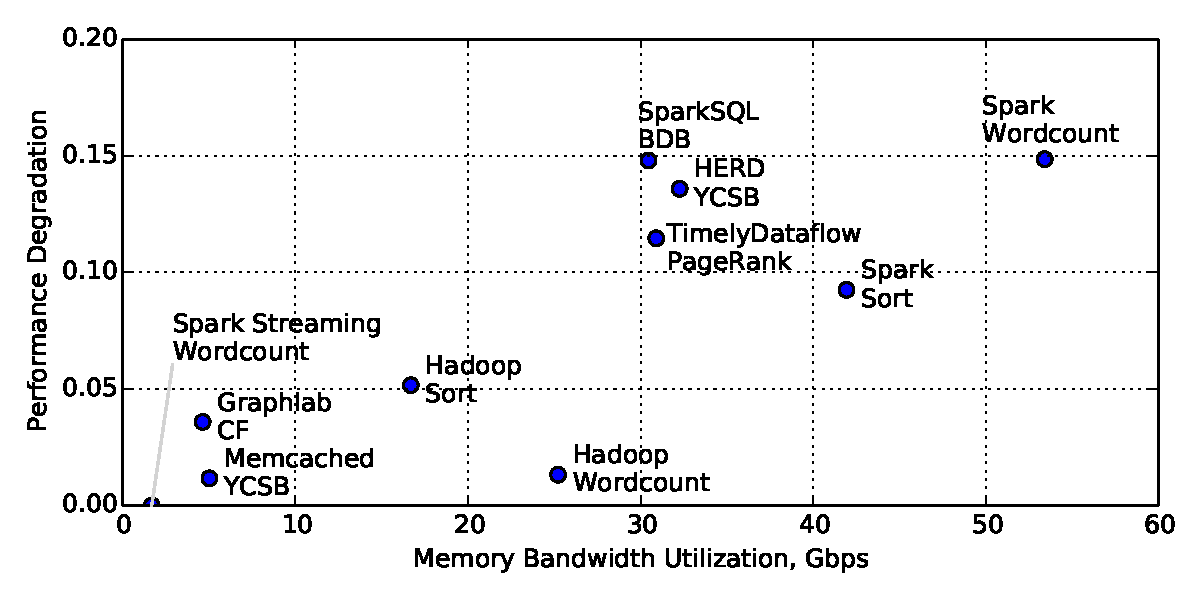
\includegraphics[width=0.95\columnwidth]{img/mem_bandwidth}
        \label{fig:memband}
    }
    \caption{\small{Performance degradation of applications is correlated with the swap memory bandwidth and overall memory bandwidth.}}
    \label{fig:bandwidths11}
\end{figure*}
%

%\vspace{-0.1in}
\subsection{Results}
\label{ssec:rr}
%\vspace{-0.05in}
We start by evaluating application performance in a disaggregated vs. a server-centric architecture. 
Figure~\ref{fig:latb} plots the performance degradation for each application under different assumptions about the latency and bandwidth to remote memory. In these experiments, we set the local memory in the disaggregated scenario to be  $25\%$ of that in the server-centric case (we will examine our choice of 25\% shortly). 
\revisionb{Note that the injected latency is constant across requests; we leave studying the effects of possibly high tail latencies to future work.}

From Figure~\ref{fig:latb}, we see that our applications can be broadly divided into two categories based on the network latency and bandwidth needed to achieve a low performance penalty.
For example, for the applications in Fig.~\ref{fig:latb} (top) --- Hadoop Wordcount, Hadoop Sort, Graphlab and Memcached --- a network with an end-to-end latency of $5\mu$s and bandwidth of $40$Gbps is sufficient to maintain an average performance penalty under 5\%. 
In contrast, the applications in Fig.~\ref{fig:latb} (bottom) --- Spark Wordcount, Spark Sort, Timely, SparkSQL BDB, and HERD --- require network latencies of $3\mu$s and $40-100$Gbps bandwidth to maintain an average performance penalty under 8\%. We term the former applications {\em \dolphin} and the latter {\em \shark} \cut{reflecting their more relaxed vs. demanding natures} and examine the feasibility of meeting their respective requirements in \S\ref{ssec:rtt}.
\revision{We found that Spark Streaming has a low memory footprint. As a result, its performance degradation is near zero in \dis, and we show it only in Figure~\ref{fig:bandwidths11}.}

\paragraphb{Sensitivity analysis}
Next, we evaluate the sensitivity of application performance to network bandwidth and latency. Fig.~\ref{fig:impbw} plots the performance degradation under increasing network bandwidth assuming a fixed network latency of $5\mu$s while Fig.~\ref{fig:impl} plots degradation under increasing latency for a fixed bandwidth of $40$Gbps; in both cases, local memory is set at $25\%$ as before.
%nd end-to-end latency to be  and varying the bandwidth from $10$Gbps to $100$Gbps (Figure~\ref{fig:impbw}). 
We see that beyond $40$Gbps, increasing network bandwidth offers little improvement in application-level performance. 
%
\cut{ 
% move to later. 
This result is in sharp contrast with existing disaggregated hardware proposals that implicitly assume the necessity of high bandwidth links using non-commodity network components (\eg, Silicon photonic~\cite{firebox, hptm, rsa}, or PCIe links~\cite{huawei}); our evaluation suggests that, for existing applications and workloads, commodity network components with $40-100$Gbps bandwidth links may be sufficient. 
}
%
In contrast, performance --- particularly for \shark apps --- is very sensitive to network latency; very low latencies ($3-5\mu$s) are needed to avoid non-trivial performance degradation.

Finally, we measure how the amount of local memory impacts application performance.
%The result of Figure~\ref{fig:latb} assumed that each CPU blade retains $25\%$ of memory capacity as local cache. We now evaluate how amount of local cache impacts the application-level performance (and hence, our conclusions) above. 
Figure~\ref{fig:impb} plots the performance degradation that results as we vary the fraction of local memory from $100\%$ (which corresponds to no CPU-memory disaggregation) down to $10\%$, assuming a fixed network latency and bandwidth of $5\mu$s and $40$Gbps respectively; note that the $25\%$ values in Figure~\ref{fig:impb} correspond to $5\mu$s, $40$Gbps results in Figure~\ref{fig:latb}. 
As expected, we see that \shark applications are more sensitive to the amount of local memory than \dolphin apps; e.g., increasing the amount of local memory from $20\%$ to $30\%$ roughly halves the performance degradation in \shark from approximately $15\%$ to $7\%$.
%even for $5\mu$s end-to-end latency. 
%In contrast, dolphin applications are far less sensitive to the amount of local memory. 
In all cases, increasing the amount of local memory beyond $40\%$ has little to no impact on performance degradation.


\paragraphb{Understanding (and extrapolating from) our results} 
One might ask \emph{why} we see the above requirements -- i.e., what characteristic of the applications we evaluated led to the specific bandwidth and latency requirements we report? Understanding these characteristics could also allow us to generalize our findings to other applications. 

%The results in Figure~\ref{fig:latb} lead to two interesting questions. First, what differentiates the dolphin applications from shark applications, and causes the variation in results across applications within a class? Second, how should one estimate the performance degradation for a new application and workload?

We partially answer this question using Figure~\ref{fig:bandwidths11}, which plots the performance degradation of the above nine workloads against their swap and memory bandwidth{\footnote{We use Intel's Performance Counter Monitor software~\cite{intel-mem-count} to read the uncore performance counters that measure the number of bytes written to and read from the integrated memory controller on each CPU. We confirmed using benchmarks designed to saturate memory bandwidth~\cite{mem-band-bench} that we could observe memory bandwidth utilization numbers approaching the reported theoretical maximum. As further validation, we verified that our Spark SQL measurement is consistent with prior work~\cite{georgeporter}.}}. Figure~\ref{fig:swapband} and~\ref{fig:memband} show that an application's performance degradation is very strongly correlated with its swap bandwidth and well correlated with its memory bandwidth. The clear correlation with swap bandwidth is to be expected. That the overall memory bandwidth is also well correlated with the resultant degradation is perhaps less obvious and an encouraging result as it suggests that an application's memory bandwidth requirements might serve as a rough indicator of its expected degradation under disaggregation: this is convenient as memory bandwidth is easily measured without requiring any of our instrumentation (i.e., emulating remote memory by a special swap device, etc.). Thus it should be easy for application developers to get a rough sense of the performance degradation they might expect under degradation and hence the urgency of rewriting their application for disaggregated contexts.

We also note that there is room for more accurate predictors: the difference between the two figures (Figs.~\ref{fig:swapband} and~\ref{fig:memband}) shows that the locality in memory access patterns does play some role in the expected degradation (since the swap bandwidth which is a better predictor captures only the subset of memory accesses that miss in local memory). Building better prediction models that account for an application's memory access pattern is an interesting question that we leave to future work. 


\eat{
The results from Figure~\ref{fig:bandwidths11} also suggest a way to generalize our results to new applications and workloads. Specifically, one can measure the swap bandwidth \rc{note that it's easier to measure memory bandwidth?} and the overall memory bandwidth for a new application and extrapolate from the results in Figure~\ref{fig:bandwidths11} to obtain a rough estimate on performance degradation for the new application and/or workload.
} 


\revision{
\paragraphb{Access Granularity}
Tuning the granularity of remote memory access is an interesting future work.
For example, soNUMA~\cite{sonuma} accesses remote memory at cache-line size granularity, which is smaller than page-size. This may allow point-query applications to optimize their dependence on remote memory.
On the other hand, developers of applications which use large, contiguous blocks of memory may use hugepages to reduce the number of page table entries and thus speed up virtual memory mapping. Since Linux currently limits (non-transparent) hugepages from being swapped out of physical memory, exploring this design option is not currently feasible.
Overall, we anticipate programmers in DDC will face a tradeoff in optimizing their applications for disaggregation depending on its memory access patterns.

\eat{
Increasing the page size (by using hugepages) can potentially reduce the number of page table entries and hence speeds up virtual memory mapping. 
So application developers tend to choose hugepage if their program uses large contiguous blocks of memory.
We anticipate that programmers in DDC will face the same tradeoff they do today in using hugepages.
That is, hugepages are chosen if the application’s memory needs warrants it and hence this should not lead to wasted use of network bandwidth.
\revisionb{
Since Linux limits (non-transparent) hugepages to be swapped out of the physical memory, paging to remote memory is not feasible currently.

soNUMA~\cite{sonuma} accesses remote memory at cache-line size granularity, which is much smaller than page-size.
Exploring the optimal granularity of remote memory access could be interesting future work.
}
}
}

\revision{
\paragraphb{Remote SSD and NVM}
Our methodology is not limited to swapping to remote memory.
In fact, as long as the 3$\mu$s latency target is met, there is no limitation on the media of the remote storage. 
We envision that the remote memory could be replaced by SSD or Non-Volatile Memory (NVM) techniques, and anticipate different price and performance tradeoff for these technologies. 
}


\paragraphb{Summary of results} 
In summary, supporting memory disaggregation while maintaining application-level performance within reasonable bounds imposes certain requirements on the network in terms of the end-to-end latency and bandwidth it must provide. Moreover, these requirements are closely related to the amount of local memory available to CPU blades. Table~\ref{tab:rmem} summarizes these requirements for the applications we studied. We specifically investigate a few combinations of network latency, bandwidth, and the amount of local memory needed to maintain a performance degradation under 5\%. 
We highlight these design points because they represent what we consider to be sweet spots in achievable targets both for the amount of local memory and for network requirements, as we discuss next.


%Next, we examine the feasibility of meeting the network requirements.
%
\cut{ 
to avoid  (has a more significant impact of application-level performance (Figure~\ref{fig:impl}). In particular, while \shark application performance is extremely sensitive to remote memory access latency, the performance for \dolphin applications can also be impacted significantly due to high latency. We use this observation below to discuss the implications and feasibility of networks for disaggregated datacenters.

\paragraphb{Impact of CPU blade density}
We start our evaluation by studying the impact of local memory on application-level performance. \rc{I am thinking about this; not sure how larger number of cores would impact the number of memory accesses!}

\paragraphb{Impact of data sizes}
We start our evaluation by studying the impact of local memory on application-level performance. \rc{I am thinking about a concise way to discuss this issue --- for Hadoop, Spark it may be easy (the number of tasks/waves increase proportionally, things should not change); for memcached and SparkSQL, unclear}

Overall, we conclude that \emph{it is possible to achieve resource disaggregation with little or no impact of application-level performance if the underlying network fabric can provide an end-to-end latency of $5\mu$s (for \dolphin applications) and of $3\mu$s (for \shark applications) along with a $40$Gbps bandwidth links}. 
} 

%
\begin{table*}[t]
  \centering
  \small{
  \begin{tabular}{c|r|r|r|r|r|r}
	\multirow{2}{*}
	    {\bf Component     } & 
	    \multicolumn{2}{c|}{\bf Baseline ($\mu$s)} & 
	    \multicolumn{2}{c|}{\bf With RDMA ($\mu$s)} & 
	    \multicolumn{2}{c}{\bf With RDMA + NIC Integr. ($\mu$s)}\\
	   	& {\bf Inter-rack} & {\bf Intra-rack} 
	   	& {\bf Inter-rack} & {\bf Intra-rack} 
	   	& {\bf Inter-rack} & {\bf Intra-rack} \\
	\hline	\hline
    OS & $2 \times 0.95$ & $2 \times 0.95$ & $0$ & $0$ & $0$ & $0$\\\hline
    Data copy & $2 \times 1.00$ &  $2 \times 1.00$ & $2 \times 1.00$ & $2 \times 1.00$ & $2 \times 0.50$ & $2 \times 0.50$\\\hline
    Switching & $6 \times 0.24$ &  $2 \times 0.24$ & $6 \times 0.24$ & $2 \times 0.24$ & $6 \times 0.24$ & $2 \times 0.24$ \\\hline
    Propagation (Inter-rack) & $4 \times 0.20$ & $0$ & $4 \times 0.20$ & $0$ & $4 \times 0.20$ & $0$\\\hline
    % (Inter-rack)&  &   & & & &\\\hline
    Propagation (Intra-rack) & $4 \times 0.02$ & $4 \times 0.02$ & $4 \times 0.02$ & $4 \times 0.02$ & $4 \times 0.02$ & $4 \times 0.02$\\ \hline
    %(Intra-rack) &  &   & & & \\\hline
    Transmission & $1 \times 0.82$ & $1 \times 0.82$ & $1 \times 0.82$ & $1 \times 0.82$ & $1 \times 0.82$ & $1 \times 0.82$\\\hline
    \hline
    {\bf Total} & {\bf $7.04\mu$s} & {$5.28\mu$s} & {$5.14\mu$s} & {$3.38\mu$s} & {\bf $4.14\mu$s} & {\bf $2.38\mu$s}\\\hline
	\hline
  \end{tabular}
  }
  \caption{\small{Achievable round-trip latency (Total) and the components that contribute to the round-trip latency (see discussion in \S\ref{ssec:rtt}) on a network with $40$Gbps access link bandwidth (one can further reduce the {\bf Total} by $0.5\mu$s using $100$Gbps access link bandwidth). The baseline denotes the latency achievable with existing network technology. The fractional part in each cell is the latency for one traversal of the corresponding component and the integral part is the number of traversal performed in one round-trip time (see discussion in \S\ref{ssec:rtt}).}}
  \label{tab:latency}
\end{table*}
%
%\vspace{-0.1in}
\subsection{Implications and Feasibility}
\label{ssec:rtt}
%\vspace{-0.05in}
We now examine the feasibility of meeting the requirements identified above. 

\paragraphb{Local memory} We start with the requirement of between $20-30$\% local memory.
In our experiments, this corresponds to between $1.50-2.25$GB/core. 
We look to existing hardware prototypes for validation of this requirement. 
Firebox targets $128$GB of local memory shared by $100$ cores leading to $1.28$GB/core,\footnote{We thank Krste Asanovi{\'c} for clarification on Firebox's technical specs.} while the analysis in ~\cite{ddcHwDesign1} uses $1.5$GB/core. 
\revision{Further, \cite{ddcHwDesign2} also indicates 25\% local memory as a desirable setting, and HP’s ``The Machine''~\cite{themachine2} uses an even larger fraction of local memory: ~87\%.
Thus we conclude that our requirement on local memory is compatible with demonstrated hardware prototypes.}
Next, we examine the feasibility of meeting our targets for network bandwidth and latency.


\paragraphb{Network bandwidth} Our bandwidth requirements are easily met: $40$Gbps is available today in commodity datacenter switches \emph{and} server NICs~\cite{40gnic}; in fact, even $100$Gbps switches and NICs are available, though not as widely~\cite{100gnic}.
Thus, ignoring the potential effects of congestion (which we consider in \S\ref{sec:existing}), providing the network bandwidth needed for disaggregation should pose no problem. Moreover, this should continue to be the case in the future because the trend in link bandwidths currently exceeds that in number of cores~\cite{hmc1, hmc2, hmc3}.


\paragraphb{Network latency} The picture is less clear with respect to latency. In what follows, we consider the various components of network latency and whether they can be accommodated in our target budget of 3$\mu$secs (for \shark apps) to 5$\mu$secs (for \dolphin apps).

Table~\ref{tab:latency} lists the six components of the end-to-end latency incurred when fetching  a $4$KB page using $40$Gbps links, together with our estimates for each. Our estimates are based on the following assumptions about existing datacenter networks: (1) the one-way path between servers in different racks crosses three switches (two ToR and one core switch) while that between servers in the same rack crosses a single ToR switch, (2) inter-rack distances of $40$m and intra-rack distances of $4$m with a propagation speed of $5$ns/m, (3) cut-through switches.\footnote{As before, we ignore the queuing delays that may result from congestion at switches -- we will account for this in \S\ref{sec:existing}.}  
With this, our round-trip latency includes the software overheads associated with moving the page to/from the NIC at both the sending and receiving endpoints (hence 2x the OS and data copy overheads), 6 switch traversals, 4 link traversals in each direction including two intra-rack and two cross-rack, and the transmission time for a 4KB page (we ignore transmission time for the page request), leading to the estimates in Table~\ref{tab:latency}. 

We start by observing that the network introduces three unavoidable latency overheads: (i) the data transmission time, (ii) the propagation delay; and (iii) the switching delay. 
Together, these components contribute to $\tilda3.14\mu$s across racks and $1.38\mu$s within a rack.\footnote{Discussions with switch vendors revealed that they are approaching the fundamental limits in reducing switching delays (for electronic switches), hence we treat the switching delay as unavoidable.} 
%, assuming cut-through switching as is the norm in commodity datacenter switches~\cite{arista,broadcom}.

In contrast, the network software at the endpoints is a significant contributor to the end-to-end latency! 
Recent work reports a round-trip kernel processing time of $950$ ns measured on a $2.93$GHz Intel CPU running FreeBSD (see ~\cite{luigi} for details), while ~\cite{ramcloud} reports an overhead of around $1\mu$s to copy data between memory and the NIC.
With these estimates, the network software contributes roughly $3.9\mu$s latency --- this represents $55\%$ of the end-to-end latency in our baseline inter-rack scenario and $73\%$ in our baseline intra-rack scenario.

The end-to-end latencies we estimated in our baseline scenarios (whether inter- or intra-rack) 
fail to meet our target latencies for either \shark or \dolphin applications. Hence, we consider potential optimizations and technologies that can reduce these latencies. 
Two technologies show promise: RDMA and integrated NICs.

%\rc{Luigi}~\cite{luigi} evaluate this latency component for a server running FreeBSD HEAD %$64$bit OS on a i$7-870$ at $2.93$GHz + Turboboost CPU with Intel $10$Gbit NIC and ixgbe %driver. The evaluation shows that the {\em average} kernel packet processing time is roughly %$950$ns at each server, leading to $1.9\mu$s for a round trip time. 
%Once the packet is processed, existing commodity NICs require copying the data from the user space to the NIC buffer, which is estimated to be around $2\mu$s per server~\cite{ramcloud}. 



\paragraphb{\emph{Using RDMA}}
RDMA effectively bypasses the packet processing in the kernel, thus eliminating the OS overheads from Table~\ref{tab:latency}.
Thus, using RDMA (Infiniband~\cite{infiniband} or \revisionb{Omnipath~\cite{omnipath}}), we estimate a reduced end-to-end latency of $5.14\mu$s across racks (column\#4 in Table~\ref{tab:latency}) 
and $3.38\mu$s within a rack.

\paragraphb{\emph{Using NIC integration}}
Recent industry efforts pursue the integration of NIC functions closer to the CPU~\cite{cpu-nic} which would reduce the overheads associated with copying data to/from the NIC. Rosenblum {\it et al.}~\cite{lowlatency} estimate that such integration with certain software  optimizations can reduce copy overheads to sub-microseconds, which we estimate at $0.5\mu$s (similar to~\cite{lowlatency}). 
%data copy from user space to NIC buffers can be reduced to sub-microseconds with the integration of NIC functions into the CPU and software optimizations~\cite{lowlatency}. 

\paragraphb{\emph{Using RDMA and NIC integration}}
As shown in column\#5 in Table~\ref{tab:latency}, RDMA together with NIC integration reduces the end-to-end latency to $4.14\mu$s across racks; within a rack, this further reduces down to $2.38\mu$s (using the same differences as in column\#2 and column\#3).

\paragraphb{Takeaways} We highlight a few takeaways here:
%
\begin{itemize}[leftmargin=*]
\itemsep0em
	\item The overhead of network \emph{software} is the key barrier to realizing disaggregation with current networking technologies. Technologies such as RDMA and integrated NICs that eliminate some of these overheads offer promise: reducing end-to-end latencies to $4.14\mu$s between racks and $2.38\mu$s within a rack. However, demonstrating such latencies in a working prototype remains an important topic for future exploration.
	\item Even assuming RDMA and NIC integration, the end-to-end latency across racks ($4.14\mu$s) meets our target latency only for \dolphin, but not \shark, applications. Our target latency for \shark apps is only met by the end-to-end latency within a rack. Thus, \shark jobs will have to be scheduled within a single rack (or nearby racks).
	That is, while \dolphin jobs can be scheduled at blades distributed across the datacenter, \shark jobs will need to be scheduled within a rack. The design and evaluation of such schedulers remains an open topic for future research.
	%Finally, even with kernel bypass, CPU-NIC integration and $100$Gbps link bandwidths, we will need intelligent schedulers for resource disaggregated datacenters. 
	\item While new network hardware such as high-bandwidth links (e.g., 100Gbps or even 1Tbps as in~\cite{vladimir, firebox}) and high-radix switches (\eg, $1000$ radix switch~\cite{firebox})  are certainly useful, they optimize a relatively small piece of the overall latency in our baseline scenario technologies. All-optical switches also fall into this category -- providing both potentially negligible switching delay and high bandwidth. That said, once we assume the benefits of RDMA and NIC integration, then the contribution of new links and switches could bring even the cross-rack latency to within our 3$\mu$sec target for \shark applications, enabling true datacenter-scale disaggregation; e.g., using $100$Gbps links reduces the end-to-end latency to $3.59\mu$s between racks, extremely close to our 3$\mu$secs. 
	%An immediate take-away is that optimizing the network software stack can lead to significantly more gains that optimizing the network hardware. In particular, using kernel bypass and CPU-NIC integration, the end-to-end latency can be reduced down to  Thus, while there is reason to believe that software overheads can be optimized to fit within our target latency budget, 
	%at the end-hosts leads to significant reduction in end-to-end latency compared to optimizations in the network fabric. Furthermore, the transmission time can be reduced to a minimal ($0.03\mu$s for $4$KB data) using $1$Tbps links. Overall, we estimate that the fundamental limits to end-to-end latency is $3.57\mu$s for inter-rack communication and $1.41\mu$s for intra-rack communication.
	\item Finally, we note that managing network congestion to achieve zero or close-to-zero queuing within the network will be essential; e.g., a packet that is delayed such that it is queued behind (say) 4 packets will accumulate an additional delay of $4\times0.82\mu$s! 
	Indeed, reducing such transmission delays may be the reason to adopt high-speed links. We evaluate the impact of network congestion in the following section.
	%SR: confused myself about this: hat necessitates One possibility is to consider adopting $100$Gbps technology \emph{not} because we need the higher capacity but instead to reduce transmission and queueing times. Using $100$Gbps links, the end-to-end latency could be reduced to $3.59\mu$s between racks and $1.83\mu$s within a rack, extremely close to our desired latency bounds.

% 	\item Somewhat surprisingly, the scope of disaggregation (i.e., rack-scale vs. datacenter-wide) is not an important factor in the feasibility of scaling disaggregation; instead, network bandwidth and an application's memory access pattern play a more important role. Our evaluation suggests that disaggregation at the scale of an entire datacenter is possible.
\end{itemize} 

% An immediate takeaway is that managing network congestion to achieve zero or close-to-zero queueing delay will be essential. This need is exacerbated by the 
% non-trivial role of transmission delays (compared to classic wide-area contexts where propagation delay dominates): e.g., a packet that is delayed such that it incurs a store-and-forward delay at each switch along a 5-hop path will accumulate an additional $4\mu$s of delay just in transmission time! 
